\documentclass[12pt]{article}

\usepackage{amsmath}
\usepackage{graphicx}
\usepackage{geometry}
\usepackage{float}
\usepackage{setspace}
\usepackage{lmodern}
\usepackage{array}
\usepackage{caption}
\usepackage{ulem}
\usepackage{xcolor}

\geometry{margin=1in}
\setstretch{1.55}
\setlength{\parskip}{0.45em}

\setlength{\arrayrulewidth}{0.8pt}
\setlength{\tabcolsep}{12pt}
\renewcommand{\arraystretch}{1.5}

\begin{document}

\begin{center}
{\Huge\bfseries Parallel and Distributed Computing}\\[2cm]
{\LARGE\bfseries Assignment 6 - Introduction to CUDA}
\end{center}

\vspace{2cm}

\noindent
{\Huge\underline{\textbf{PART A}}}

\vspace{0.5cm}

{\Large\textbf{Device Query}}

\vspace{1cm}

\textbf{Ques :}

Write the device query code, compile and run it on your system. Query enough information to know all the details of your device like GPU name, compute capabilities, max block and grid dimensions, memory sizes, warp size etc.

\vspace{0.6cm}

\textbf{\Large \underline{Method}}

\vspace{0.5cm}

We use \texttt{cudaGetDeviceProperties()} to query all the GPU details. The code queries the device count first, then loops through each device and prints all the properties.

\vspace{0.5cm}

\begin{figure}[H]
\centering
\fbox{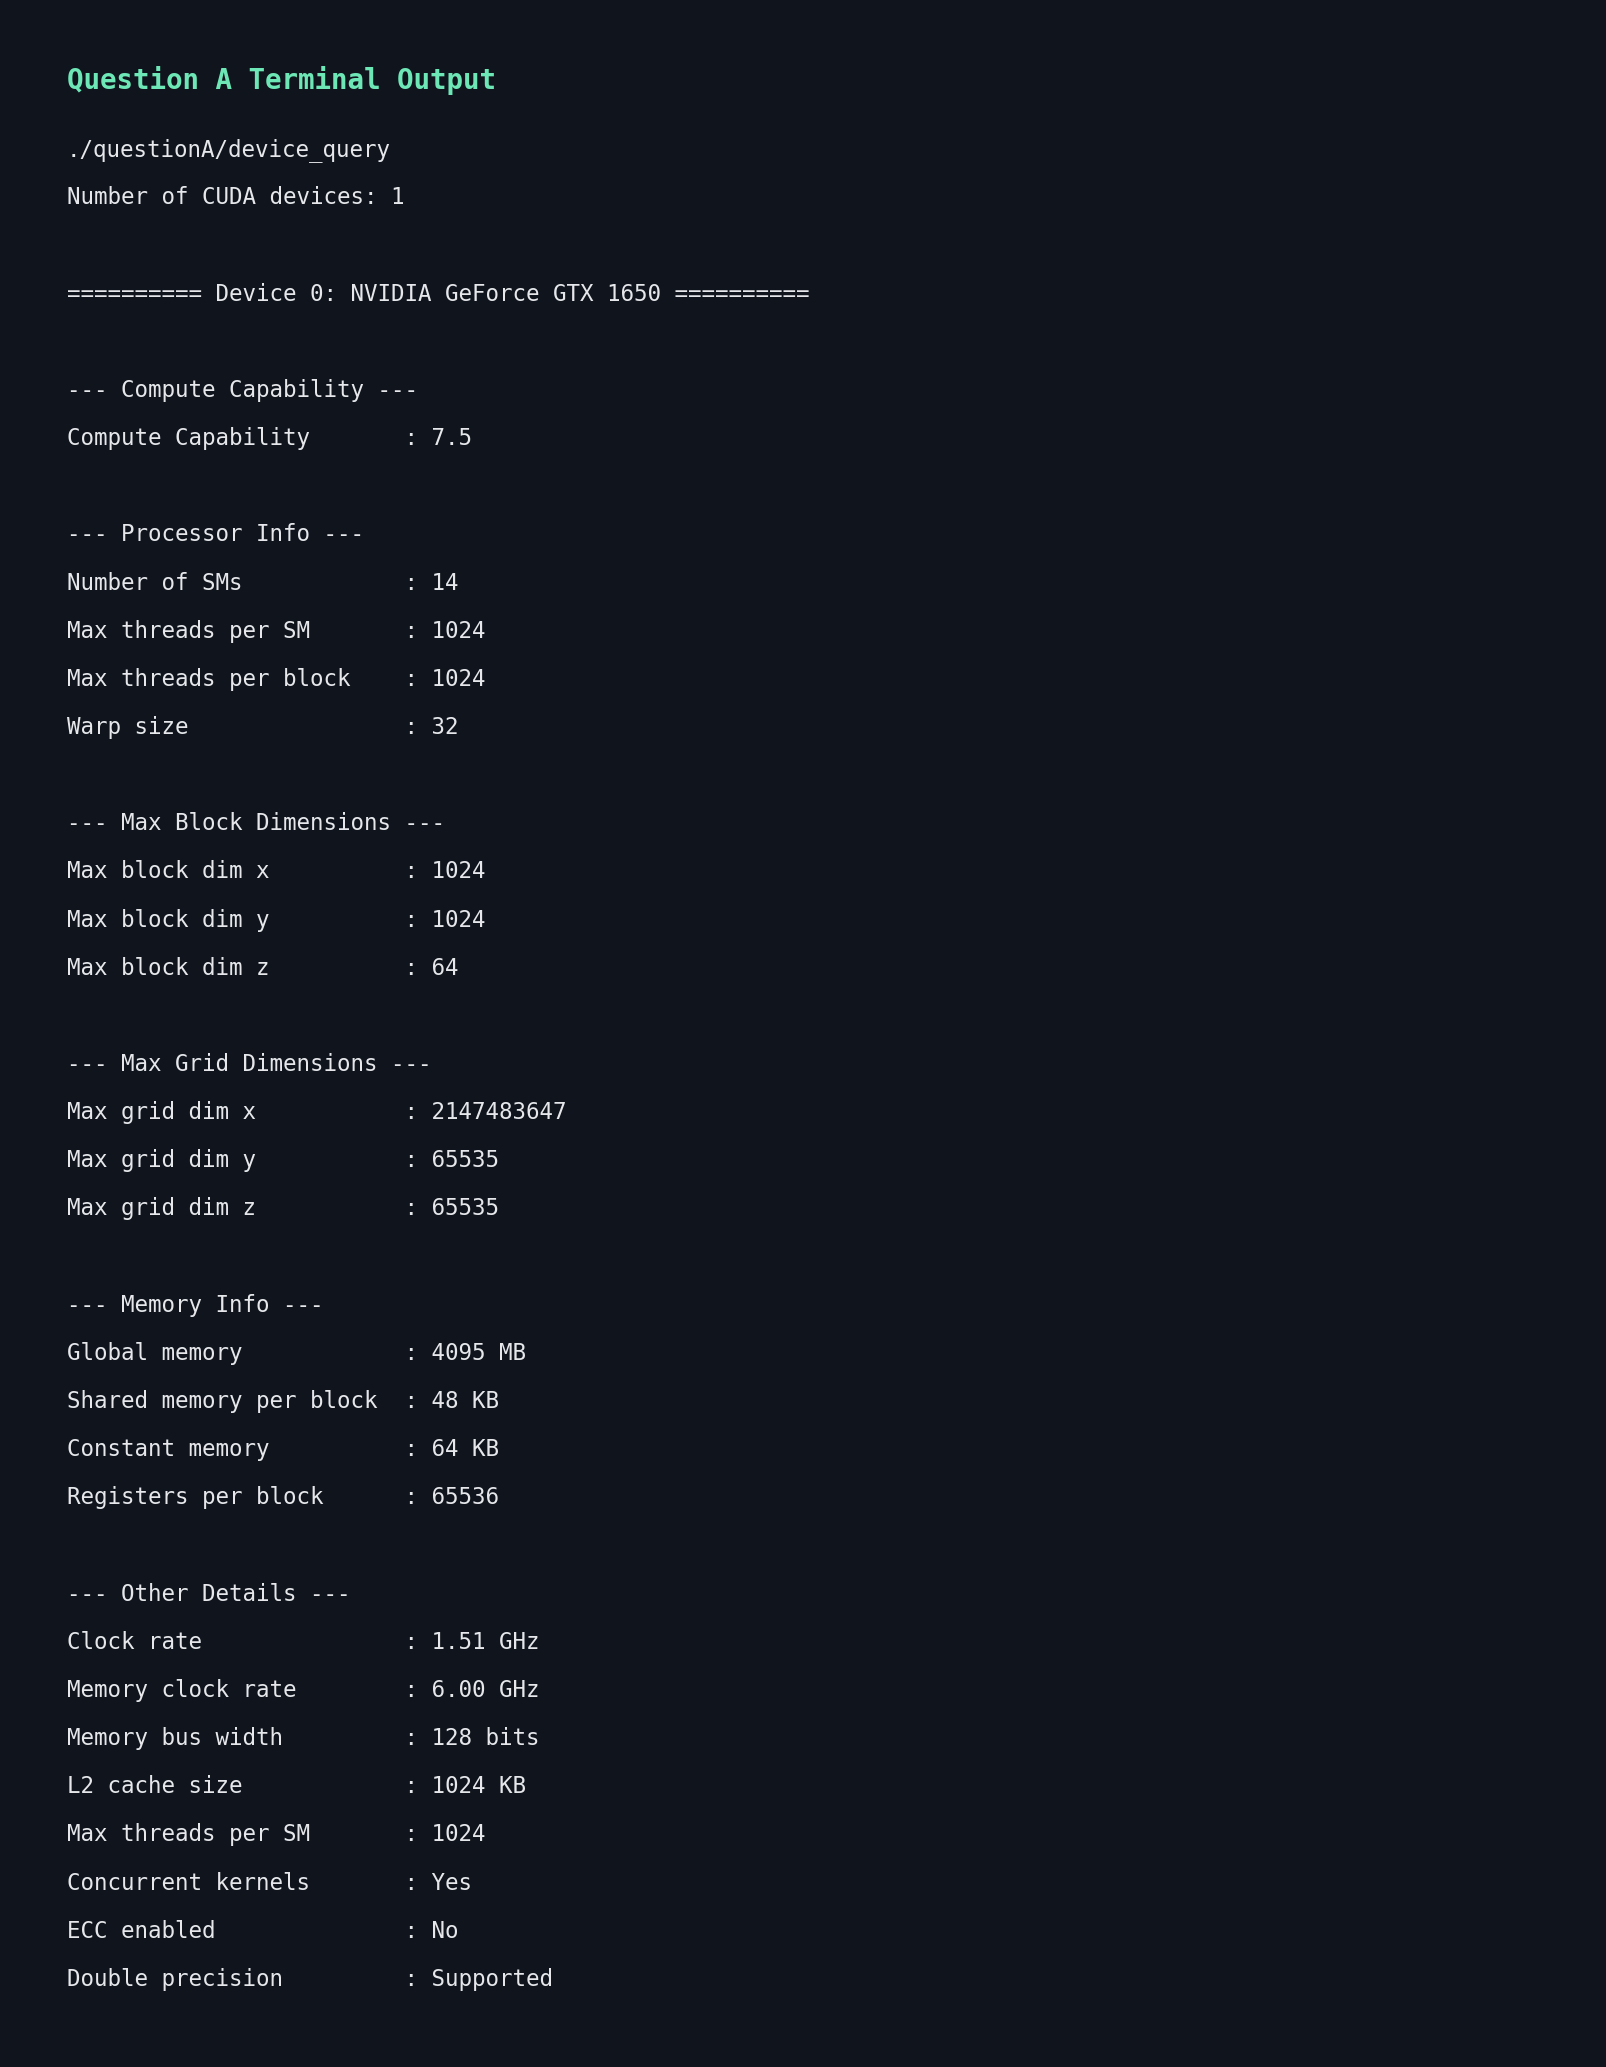
\includegraphics[width=0.9\textwidth]{outputs/outputA.png}}
\caption*{\textbf{Figure A: Device Query Output}}
\end{figure}

\vspace{1cm}

\textbf{\Large \underline{Answers to Questions}}

\vspace{0.8cm}

\textbf{1. What is the architecture and compute capability of your GPU?}

\vspace{0.3cm}

The compute capability of a GPU tells us what generation of NVIDIA architecture it belongs to and what features it supports. A higher number means newer architecture. For example compute capability 7.5 means Turing, 8.6 means Ampere, 8.9 means Ada Lovelace etc.

My GPU: NVIDIA GeForce GTX 1650 (Turing architecture, compute capability 7.5)

\vspace{0.5cm}

\textbf{2. What are the maximum block dimensions for your GPU?}

\vspace{0.3cm}

Block dimensions tell us the max number of threads we can have in each direction (x, y, z) of a thread block. But the total threads per block cant exceed the max threads per block limit which is usually 1024 on modern GPUs.

From our device query:

\begin{center}
\begin{tabular}{|p{4cm}|p{4cm}|}
\hline
\textbf{Dimension} & \textbf{Max Value} \\
\hline
Block dim x & 1024 \\
\hline
Block dim y & 1024 \\
\hline
Block dim z & 64 \\
\hline
Max threads/block & 1024 \\
\hline
\end{tabular}
\end{center}

\vspace{0.5cm}

\textbf{3. If max grid dim is 65535 and max block dim is 512, what is the max number of threads?}

\vspace{0.3cm}

For a 1D launch:

max threads = max grid dimension $\times$ max block dimension

= 65535 $\times$ 512

= \textbf{33,553,920 threads}

So roughly 33.5 million threads can be launched in a 1D grid+block configuration.

\vspace{0.5cm}

\textbf{4. Under what conditions might a programmer choose not to launch the max number of threads?}

\vspace{0.3cm}

\begin{itemize}
\item if the problem size is small - like if you only have 1000 elements to process then launching 33 million threads is pointless. most threads would sit idle doing nothing

\item if each thread needs a lot of registers or shared memory. launching too many threads means each one gets less resources and the GPU might not have enough to actually run them

\item if threads need to synchronize a lot. more threads means more synchronization overhead which can slow things down

\item sometimes using fewer threads where each thread does more work (thread coarsening) gives better performance because of less launch overhead and better cache usage
\end{itemize}

\vspace{0.5cm}

\textbf{5. What can limit a program from launching the max number of threads?}

\vspace{0.3cm}

\begin{itemize}
\item \textbf{register pressure} - GPU has a fixed number of registers per SM. if each thread uses too many registers, fewer threads can be active at the same time

\item \textbf{shared memory usage} - if a block uses too much shared memory then fewer blocks can fit on an SM simultaneously

\item \textbf{problem size} - no point launching more threads than data elements you have

\item \textbf{max threads per block} - even if the grid can be huge, each block has a hard limit (usually 1024)

\item \textbf{hardware limits} - number of SMs, max warps per SM, max blocks per SM all put a cap on occupancy
\end{itemize}

\vspace{0.5cm}

\textbf{6. What is shared memory? How much shared memory is on your GPU?}

\vspace{0.3cm}

Shared memory is a small but very fast on-chip memory that is shared between all threads in a block. Think of it like a user-managed L1 cache. Its way faster than global memory (roughly 100x faster) because its physically on the chip right next to the processing cores.

Threads in the same block can use shared memory to share data with each other and communicate. Its really useful for things like parallel reduction (like our array sum in part B) where threads need to combine their results.

Shared memory per block on my GPU: 48 KB

\vspace{0.5cm}

\textbf{7. What is global memory? How much global memory is on your GPU?}

\vspace{0.3cm}

Global memory is the main memory of the GPU - the big VRAM you see on the spec sheet. Its the largest memory available but also the slowest. All threads from all blocks can read and write to it.

When we do \texttt{cudaMalloc}, the memory gets allocated in global memory. Data has to be copied from CPU RAM to GPU global memory using \texttt{cudaMemcpy} before the GPU can work on it.

Global memory on my GPU: 4096 MB

\vspace{0.5cm}

\textbf{8. What is constant memory? How much constant memory is on your GPU?}

\vspace{0.3cm}

Constant memory is a special read-only memory on the GPU. Its cached so reads are fast (as fast as registers if all threads in a warp read the same address). But you cant write to it from a kernel - you set the values from the CPU side before launching the kernel.

Good for things like physical constants, lookup tables, kernel parameters that all threads need to read but nobody changes.

Constant memory is always \textbf{64 KB} on all CUDA GPUs - thats a fixed hardware limit.

\vspace{0.5cm}

\textbf{9. What does warp size signify? What is your GPU's warp size?}

\vspace{0.3cm}

Warp size is the number of threads that execute together in lockstep on the GPU. The GPU doesnt execute threads one at a time - it executes a whole warp (group of threads) together. All threads in a warp run the same instruction at the same time. This is called SIMT (Single Instruction Multiple Threads).

If threads in a warp take different paths in an if-else statement, the warp has to execute both paths one after another. This is called \textbf{warp divergence} and its bad for performance because half the threads sit idle during each path.

Warp size on all NVIDIA GPUs: \textbf{32 threads}

\vspace{0.5cm}

\textbf{10. Is double precision supported on your GPU?}

\vspace{0.3cm}

Double precision (64-bit float) is supported on GPUs with compute capability 1.3 and above. So basically all modern GPUs support it. But the performance is usually much worse than single precision:

\begin{itemize}
\item on consumer GPUs like GeForce - double precision runs at 1/32 the speed of single precision
\item on workstation GPUs like Tesla/A100 - its much better, about 1/2 the speed
\end{itemize}

Yes, double precision is supported on this GPU.

\newpage

\noindent
{\Huge\underline{\textbf{PART B}}}

\vspace{0.5cm}

{\Large\textbf{Array Sum using CUDA}}

\vspace{1cm}

\textbf{Ques :}

Write a CUDA program to calculate the sum of elements in a single precision float array. Follow these steps: allocate device memory, copy host to device, set up block/grid dimensions, invoke kernel, copy results back, free device memory, and write the reduction kernel.

\vspace{0.6cm}

\textbf{\Large \underline{Approach}}

\vspace{0.5cm}

We use parallel reduction in shared memory. The idea is simple - each block loads its chunk of the array into shared memory, then we do a tree-based reduction where we keep halving the active threads and adding pairs together. At the end, thread 0 of each block has the sum of that blocks elements. Then we copy all the block sums back to CPU and add them up.

\vspace{0.5cm}

\textbf{Step by step:}

\begin{enumerate}
\item \textbf{Allocate device memory} - \texttt{cudaMalloc} for the input array and an array to hold each blocks partial sum

\item \textbf{Copy host memory to device} - \texttt{cudaMemcpy} with \texttt{cudaMemcpyHostToDevice} copies our input array from CPU RAM to GPU global memory

\item \textbf{Initialize thread block and kernel grid dimensions} - we use 256 threads per block. grid size = ceil(N / blockSize) so every element gets exactly one thread

\item \textbf{Invoke CUDA kernel} - launch with shared memory size = blockSize * sizeof(float). the kernel does tree reduction inside each block

\item \textbf{Copy results from device to host} - \texttt{cudaMemcpy} with \texttt{cudaMemcpyDeviceToHost} copies the block sums back to CPU

\item \textbf{Free device memory} - \texttt{cudaFree} releases the GPU memory we allocated

\item \textbf{The kernel} - uses \texttt{extern \_\_shared\_\_ float sdata[]} for fast reduction within each block
\end{enumerate}

\vspace{0.5cm}

\vspace{0.7cm}

\begin{figure}[H]
\centering
\fbox{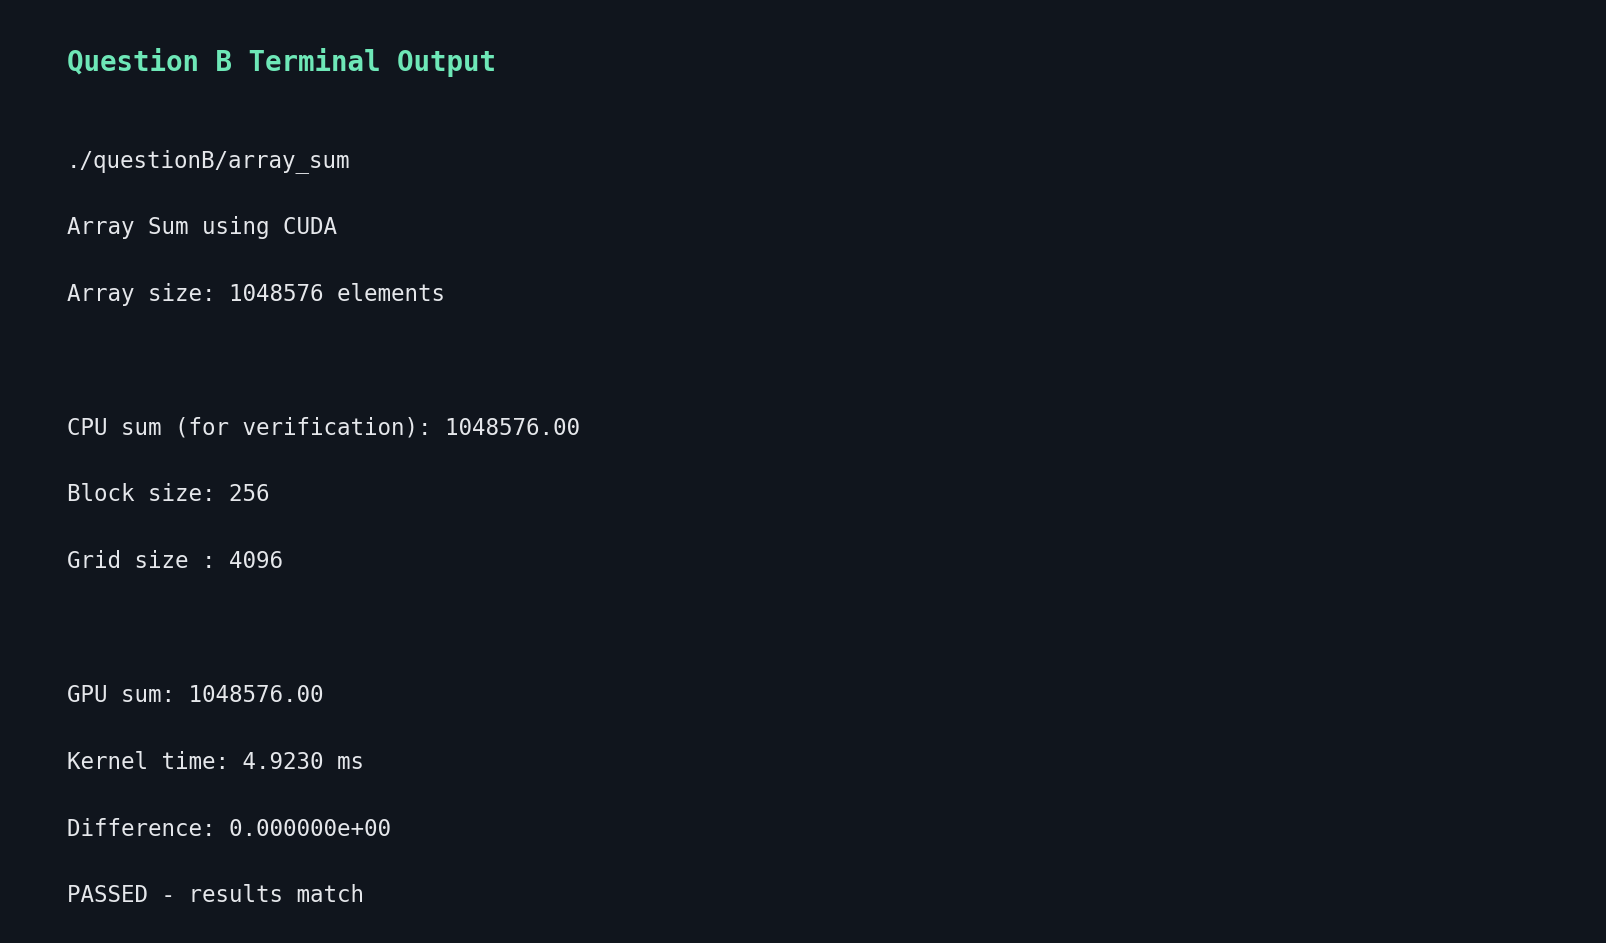
\includegraphics[width=0.9\textwidth]{outputs/outputB.png}}
\caption*{\textbf{Figure B: Array Sum Output}}
\end{figure}

\newpage

\noindent
{\Huge\underline{\textbf{PART C}}}

\vspace{0.5cm}

{\Large\textbf{Matrix Addition using CUDA}}

\vspace{1cm}

\textbf{Ques :}

Perform matrix addition of two large integer matrices in CUDA. Answer questions about floating point operations, global memory reads, and global memory writes.

\vspace{0.6cm}

\textbf{\Large \underline{Approach}}

\vspace{0.5cm}

Matrix addition is embarrassingly parallel - each element is independent. We use a 2D grid and 2D blocks to map threads directly to matrix elements. Each thread computes C[i][j] = A[i][j] + B[i][j].

We use 16x16 thread blocks (256 threads total per block) and calculate the grid dimensions to cover the entire matrix.

\vspace{0.5cm}

\vspace{0.7cm}

\begin{figure}[H]
\centering
\fbox{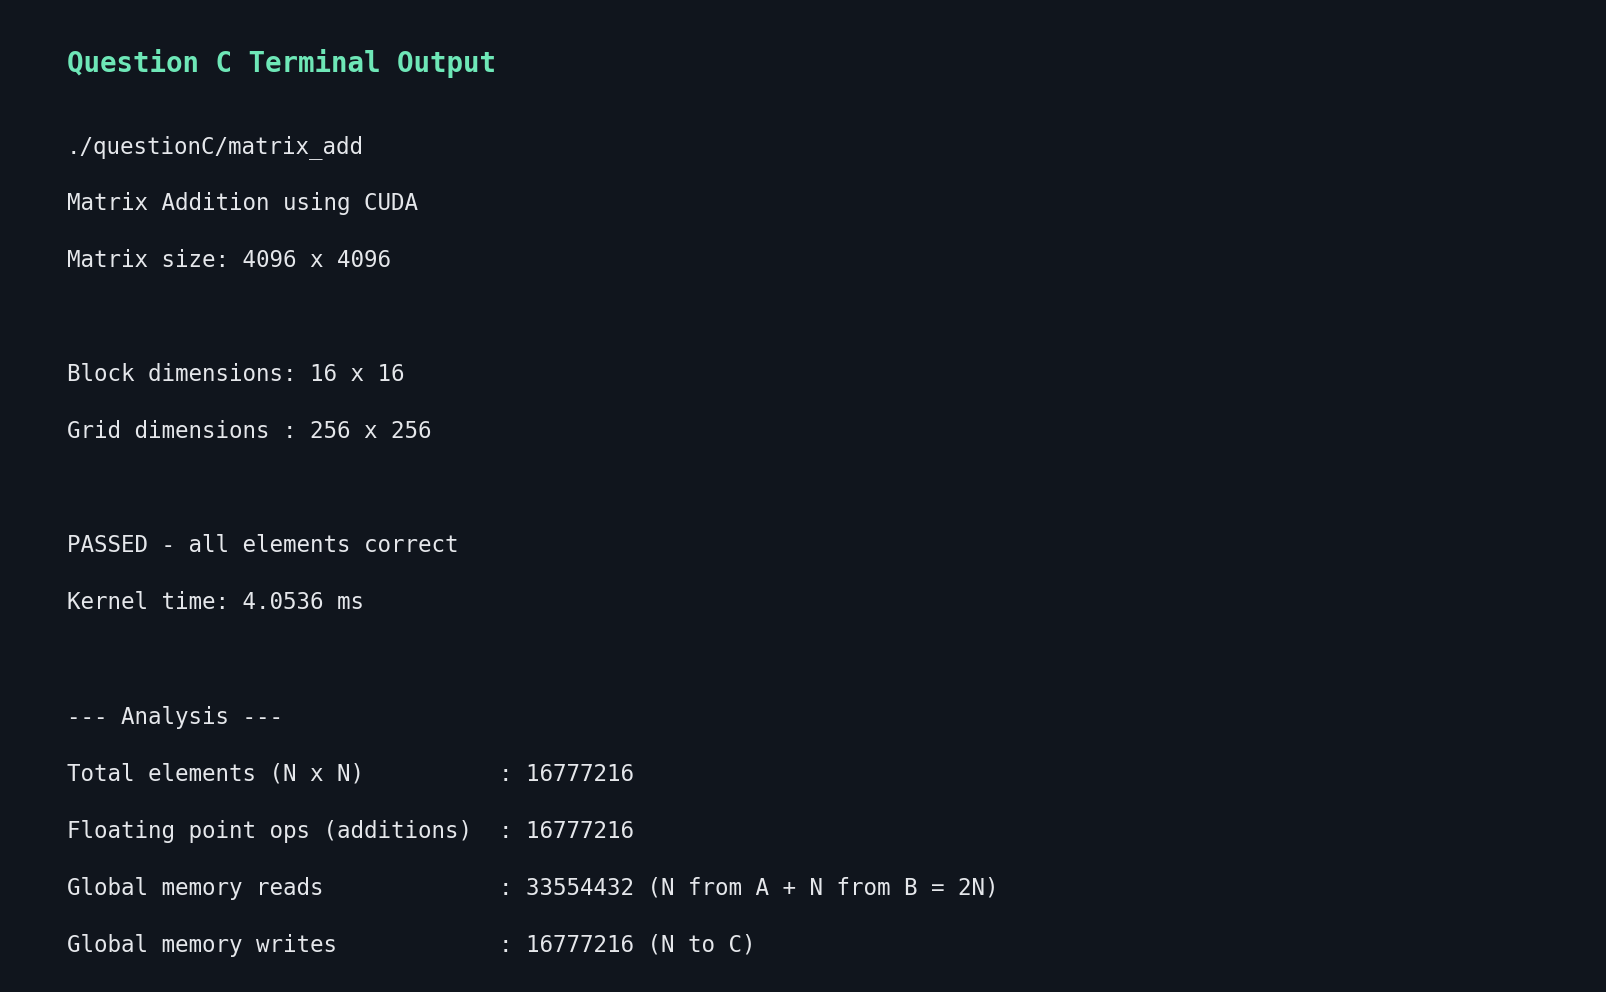
\includegraphics[width=0.9\textwidth]{outputs/outputC.png}}
\caption*{\textbf{Figure C: Matrix Addition Output}}
\end{figure}

\vspace{1cm}

\textbf{\Large \underline{Answers to Questions}}

\vspace{0.8cm}

For a matrix of size N $\times$ N where N = 4096:

\vspace{0.5cm}

\textbf{1. How many floating point operations are being performed in the matrix addition kernel?}

\vspace{0.3cm}

Each element needs exactly 1 addition operation.

Total operations = N $\times$ N = 4096 $\times$ 4096 = \textbf{16,777,216 operations}

(note: technically these are integer additions since we use int matrices but the concept is the same)

\vspace{0.5cm}

\textbf{2. How many global memory reads are being performed by your kernel?}

\vspace{0.3cm}

For each element we read:
\begin{itemize}
\item 1 element from matrix A (global memory read)
\item 1 element from matrix B (global memory read)
\end{itemize}

Total reads = 2 $\times$ N $\times$ N = 2 $\times$ 4096 $\times$ 4096 = \textbf{33,554,432 reads}

\vspace{0.5cm}

\textbf{3. How many global memory writes are being performed by your kernel?}

\vspace{0.3cm}

For each element we write:
\begin{itemize}
\item 1 element to matrix C (global memory write)
\end{itemize}

Total writes = N $\times$ N = 4096 $\times$ 4096 = \textbf{16,777,216 writes}

\vspace{0.5cm}

\begin{center}
\begin{tabular}{|p{5cm}|p{4cm}|p{4cm}|}
\hline
\textbf{Metric} & \textbf{Formula} & \textbf{Value (N=4096)} \\
\hline
Arithmetic operations & N $\times$ N & 16,777,216 \\
\hline
Global memory reads & 2 $\times$ N $\times$ N & 33,554,432 \\
\hline
Global memory writes & N $\times$ N & 16,777,216 \\
\hline
Total memory accesses & 3 $\times$ N $\times$ N & 50,331,648 \\
\hline
Arithmetic intensity & ops / mem accesses & 1/3 \\
\hline
\end{tabular}
\end{center}
\vspace{0.2cm}
\begin{center}
\textbf{Table 1: Memory access analysis for matrix addition}
\end{center}

\vspace{0.5cm}

The arithmetic intensity is only 1/3 which is very low. This means matrix addition is a \textbf{memory-bound} operation - the GPU spends most of its time moving data around and very little time doing actual computation. Compare this with matrix multiplication where the arithmetic intensity is O(N) which makes it compute-bound and much better suited for GPUs.

\vspace{0.8cm}

\begin{figure}[H]
\centering
\fbox{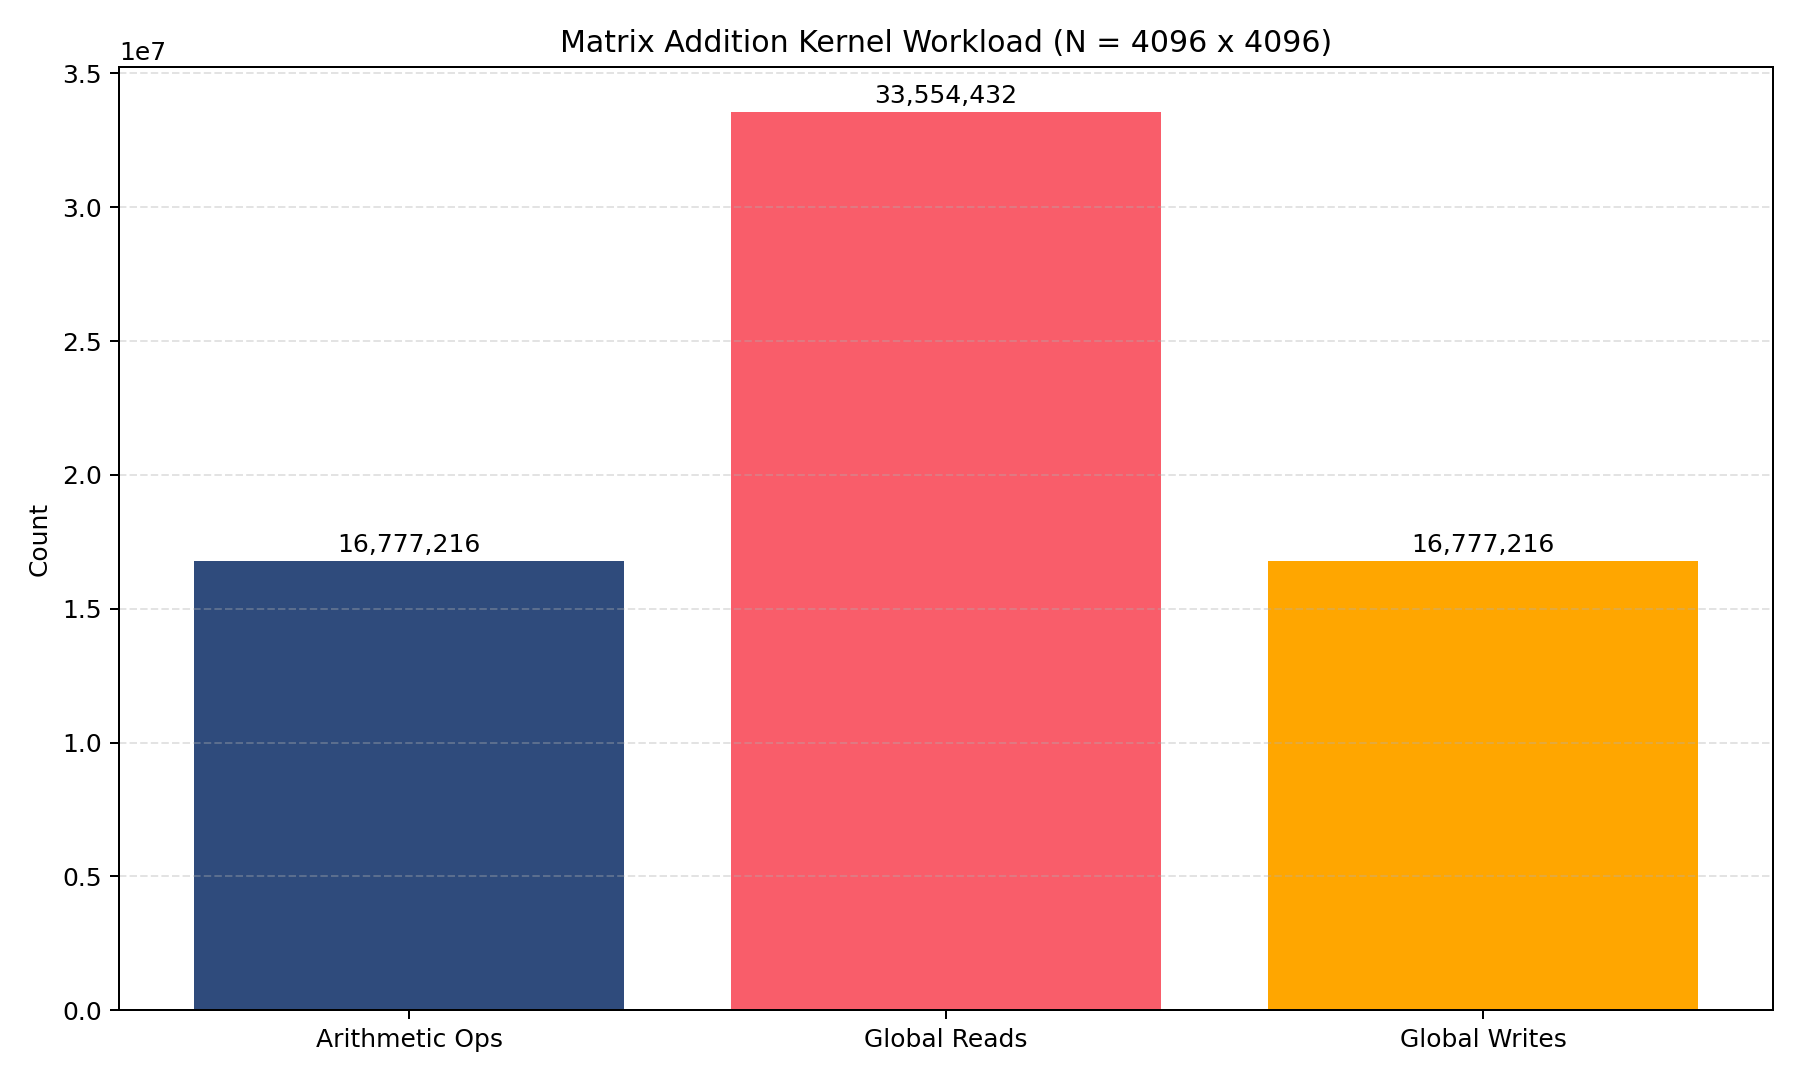
\includegraphics[width=0.85\textwidth]{outputs/outputC_ops.png}}
\caption*{\textbf{Figure D: Matrix Addition Workload Graph}}
\end{figure}

\begin{figure}[H]
\centering
\fbox{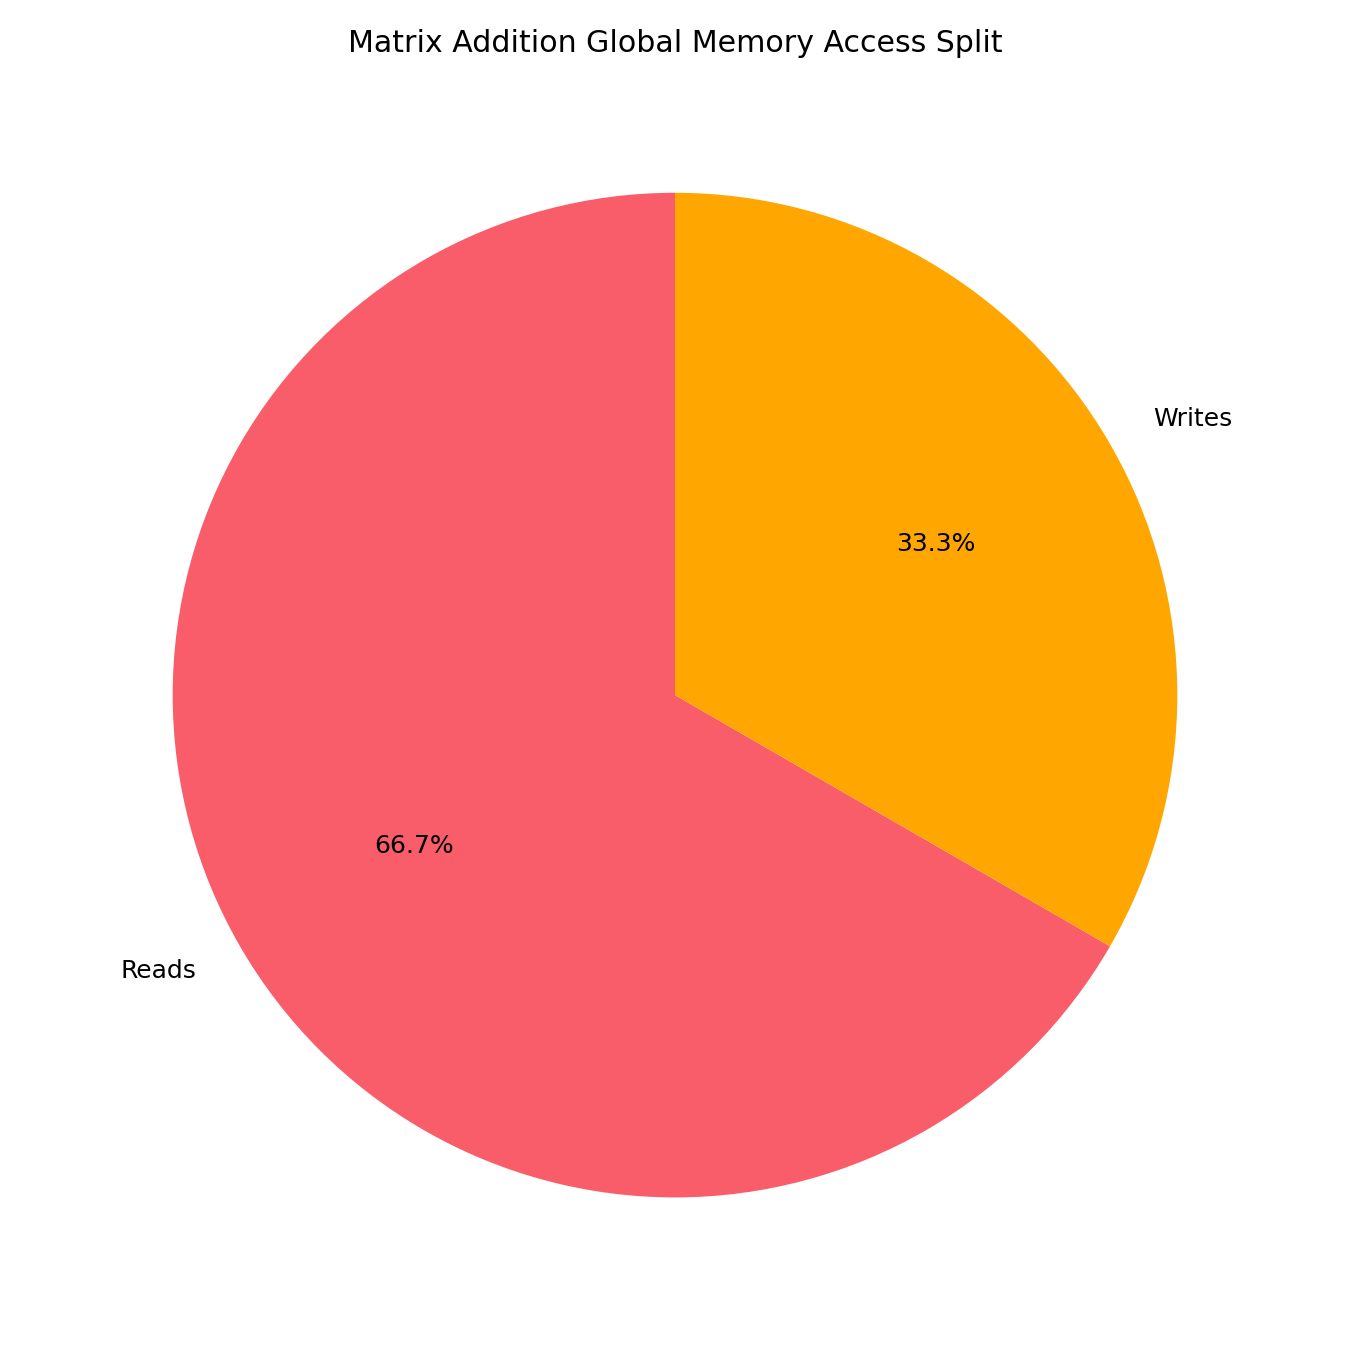
\includegraphics[width=0.62\textwidth]{outputs/outputC_memory_split.png}}
\caption*{\textbf{Figure E: Matrix Addition Memory Access Split}}
\end{figure}

\newpage

\textbf{\Large \underline{Observations}}

\vspace{1cm}

1. \textbf{CUDA programming follows a standard pattern} - allocate on GPU, copy data over, launch kernel, copy results back, free GPU memory. this host-device data transfer is often the bottleneck, not the actual computation

2. \textbf{Thread block size of 256 works well as a default} - its a multiple of the warp size (32), gives good occupancy on most GPUs, and balances register/shared memory usage. 16x16 blocks work great for 2D problems like matrix operations

3. \textbf{Shared memory reduction is much faster than naive approaches} - for the array sum, doing reduction in shared memory avoids millions of slow global memory accesses. the tree reduction pattern (halving active threads each step) does log2(blockSize) steps instead of blockSize steps

4. \textbf{Matrix addition is too simple to fully utilize a GPU} - with arithmetic intensity of 1/3, the GPU cores are mostly waiting for memory. This is why matrix multiplication (which reuses data heavily) shows much better GPU speedups

5. \textbf{Boundary checking is important} - when the array or matrix size doesnt divide evenly by the block size, some threads will be out of bounds. The \texttt{if (i < n)} check prevents illegal memory accesses

\vspace{1cm}

\textbf{\Large \underline{Inferences}}

\vspace{1cm}

1. \textbf{GPUs are best for compute-heavy parallel problems} - matrix addition doesnt benefit much from GPU because its memory-bound. but problems like matrix multiplication, deep learning, simulations etc where each data element needs lots of computation are where GPUs really shine

2. \textbf{Memory hierarchy matters a lot} - just like CPU caches, using shared memory instead of global memory can give massive speedups. our reduction kernel would be way slower if we did everything in global memory

3. \textbf{Warp-level thinking is important} - since 32 threads execute together, things like warp divergence (branching within a warp) and memory coalescing (adjacent threads accessing adjacent memory) directly impact performance

4. \textbf{The host-device transfer overhead} - for small problems, the time spent copying data between CPU and GPU can be more than the computation itself. CUDA is worth it only when the computation is heavy enough to offset this transfer cost

5. \textbf{Occupancy isnt everything} - launching more threads doesnt always mean better performance. sometimes fewer threads with more work per thread (thread coarsening) gives better results because of reduced overhead and better cache utilization

\vspace{2cm}

\textbf{Submitted to :} Dr Saif Nalband

\textbf{Submitted by :} Arpan Goyal

\textbf{Roll No. :} 102303479

\end{document}
